\section{Organizing People and Work}
\label{sec:global}

Globalization and the implicit challenges of distributed development have
become the norm in recent years for large enterprises~\cite{glo24,glo26}.
Evaristo~\cite{glo27} categorizes the nature of these challenges into five
critical areas: perceived distance (geographical and temporal), national
culture (languages, accepted work patterns), development methodology
(similarity in processes), task structure (clarity and structure to team
hand-offs) and organizational distance. The premise is that as the distance
between the teams along these critical dimensions increases, the overhead and
difficulties associated with distributed development become more
prominent. Collaborative development platforms that promote structured
interaction between team members can help make distributed development more
efficient~\cite{glo28,glo29}. Sharing expertise and the ability to leverage
best practices across engagements is a key part of ensuring efficient
collaboration -- Expertise Browser~\cite{glo30} and Hipikat~\cite{glo31} are
examples of tools that enable sharing at the level of processes and
artifacts. Given the rapid churn of resources in the global workforce, a push
model of delivering information in situ to developers is important and many of
the proposed tools~\cite{glo29,glo31} support this model. The adoption of
Cloud, API centric approach to development and agile methods are also helping
to reduce the inefficiencies inherent in distributed development. Tooling that
can help efficiently leverage a global workforce remains an active and
important area of research.

The existing literature on distributed development has mostly focused on the
need of one organization engaged in carrying out work globally for reasons
of efficiency and cost.  Services companies have additional concerns.  They
serve multiple large clients, and the work of each of those clients has to
be carried out in the distributed fashion.  In the earlier days, services
companies grew essentially distinct teams to serve distinct clients.  This
turns out to be not optimimal from a resource utilization point of view.

Recent trend has been towards \textit{competency centers}, which are virtual
entities that specialize in a specific software skill set.  The advantages of
competency center approach are resource multiplexing as well as specialization.
For example, a testing competency center could serve multiple clients, and
could be the home for testing expertise within the company. 

IBM has been a pioneer in
this field---their approach to structured delivery of IT services by a globally
distributed delivery team is called Application Assembly
Optimization~\cite{gloaao}. Other major IT services companies have adopted
variations of this approach.

\textit{Work envelopes} are the central construct in the competency-center approach for
structured delivery of software projects that enable disparate competency
centers to come together on-demand, in the context of a client engagement.  Work
envelopes represent a standard communication vehicle between distributed teams
by which each work order is authored, transported, and delivered. Work envelopes
include workflow, instruction (normative guidance), metrics collection, and risk
management/exception handling mechanisms. Each work envelope constitutes a
subset of activities that are bound to a larger project-wide work-breakdown
structure managed through a traditional project-management tool. 



%\textbf{Prior Material}
%
%The last few years have seen an accelerated trend toward organizations utilizing
%a globally integrated development model for complex IT solution
%implementation. In the first wave of the move toward globally integrated
%development, the emphasis was on reducing cost through labor arbitrage.  The
%competition among the major industry players generated the need for aggressive
%differentiation beyond lower cost---improving quality and reducing
%time-to-market also became important factors. However, traditional project
%management techniques that work well with small co-located teams do not scale
%well to a global workforce.  To be effective, the development process should be
%supplemented by an over-arching procedural and architectural framework that
%implicitly partitions the development process for effective globally sourced
%development. Formal process modeling, strict enforcement of process controls,
%and monitoring the software development process have long been touted as the
%right way to streamline global delivery~\cite{glo32}.
%
%\begin{figure}[t]
%\centering
%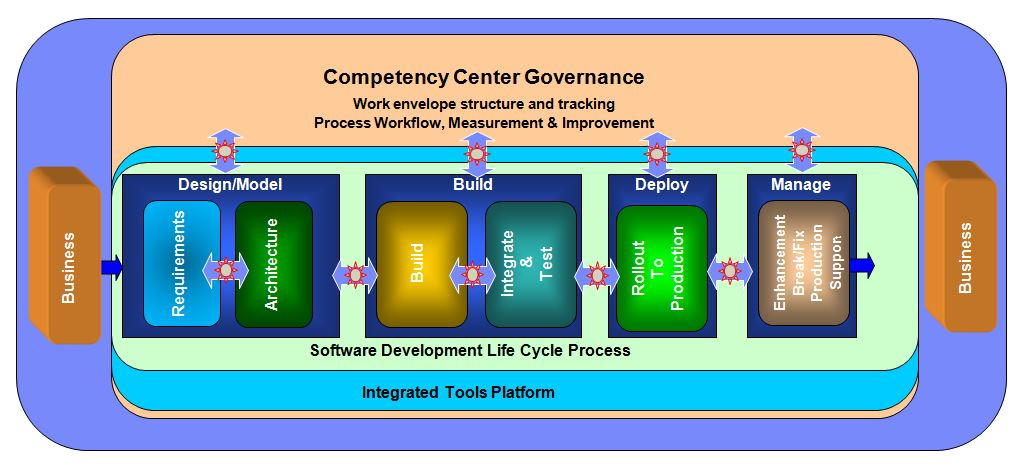
\includegraphics[bb= 28 0 740 355, scale=0.32]{figs/glocomp.jpg}
%\vspace*{-13pt}
%\caption{The globally integrated development model with competency centers.}
%\vspace*{-16pt}
%\label{glofig1}
%\end{figure}
%
%As large enterprises adapted traditional software delivery models to distributed
%development, the natural tendency has been to establish competency centers that
%cater to specific software-skill needs. The adoption of a disciplined model for
%delivery has resulted in new organizational efficiency, reduced process
%variance, and improved execution discipline. Consider the delivery of a large IT
%project that involves distributed teams with hundreds of people working on tight
%schedules to deliver mission-critical software. Many such projects fail to
%deliver on time and within budget because of the significant overhead involved
%in discovering the roles and responsibilities of teams, establishing
%communication protocols, and determining how software will be assembled, tested,
%and deployed at the client site. Competency centers that standardize key stages
%of the delivery process
%%% for customization of software from major vendors
%can reduce this overhead significantly.
%%% for a majority of enterprise-class IT projects.
%
%Figure~\ref{glofig1} shows the vision of the globally integrated enterprise by
%focusing on one of the key pain points that inhibit this vision---a structured
%way of distributing work to remote teams that promotes collaboration and
%enforces good governance practices.  Some of the key organizational entities in
%this approach include governance and operations teams, a design center that
%builds the architecture in support of client requirements, and the
%\textit{competency centers} that deliver the work. IBM has been a pioneer in
%this field---their approach to structured delivery of IT services by a globally
%distributed delivery team is called Application Assembly
%Optimization~\cite{gloaao}. Other major IT services companies have adopted
%variations of this approach.
%
%Work envelopes are central constructs in the competency-center approach for
%structured delivery of software projects that enable disparate competency
%centers to come together on-demand, in the context of a client engagement.  Work
%envelopes represent a standard communication vehicle between distributed teams
%by which each work order is authored, transported, and delivered. Work envelopes
%include workflow, instruction (normative guidance), metrics collection, and risk
%management/exception handling mechanisms. Each work envelope constitutes a
%subset of activities that are bound to a larger project-wide work-breakdown
%structure managed through a traditional project-management tool.
%
%\textbf{End of Prior material}

\subsection{Research Topic: Efficient Competency Centers}

Although the competency-center model has now become central to many IT vendors
and large enterprises, it has seen less interest in literature as the focus is
on large-scale development with a global workforce, which is hard to replicate
in an academic setting. However, there are several accessible research problems
that can significantly improve the performance of these competency centers. We
highlight five such problem areas below

\begin{enumerate}

\item Work envelopes: Central to the concept of a competency center is the
  ability to partition software projects into granular work envelopes. For
  certain classes of development and maintenance activities---for example, in
  the area of packaged applications---partitioning is natural because tasks are
  repeatable and the skill requirements for a class of tasks is easy to
  establish. Is there an equivalent construct for more complex software
  development?

\item Measurement: In a large competency center, performance measurement is key
  to ensuring efficient operation. In some ways, a competency center, due to the
  repeatable and comparable nature of tasks it undertakes, makes performance
  measurement easier. However, we find that the information reported by the
  practitioners of a competency center is often unreliable due to the complex
  structure of incentives involved. Can we leverage the structure of a
  competency center to automate the collection of information, thereby improving
  its reliability? Can we create checks and balances in information collection
  to validate performance measurement?

\item Estimation: Competency centers deal with large volumes of repeatable tasks
  belonging to a few categories that are performed by dedicated teams. We
  observed that this typically reduces the variance in the estimated time
  required to perform these tasks. The reduction in variance is a consequence of
  the predicability of the inputs and outputs of the tasks, standardized
  process, and a community of developers who can share experiences and
  know-how. In turn, this improves our ability significantly to predict the
  effort needed to complete complex software projects.

\item Governance: Enterprises have extended traditional project management
  techniques to include competency centers. However, it is unclear whether a
  project-centric governance model provides the right set of checks and balances
  to manage efficiently the output of a distributed workforce that is working on
  several projects simultaneously.

\item Planning and scheduling: Traditional calendar-day project planning is
  highly inefficient in the context of a competency center because development
  tasks can finish ahead of or behind schedule. Because a practitioner is not
  tied to a particular project in a competency center, calendar-day planning
  requires constant replanning to ensure that we are fully utilizing available
  capacity. A better approach would be to use a queue-based model, where the
  queue is managed centrally to re-prioritize the tasks in a practitioner's
  queue to ensure on-time delivery. From the practitioner's perspective, they
  move to the next task in the queue after completing the task at hand---if
  they fall behind schedule, the remaining tasks in their queue can be moved to
  other practitioners.

\end{enumerate}

\subsection{Toward Distributed Marketplaces}

The logical evolution of the competency center model that we discussed in the
last section is to extend beyond traditional organizational boundaries---in
essence, towards a competitive distributed services marketplace. Instances of
such marketplaces are already appearing; for example, services that provide
coding expertise for hire, such as RentACoder ({\small
  \url{www.rentacoder.com}}) and TopCoder ({\small \url{www.topcoder.com}}) are
simple examples of this model. Currently, these are seen as a novelty and, thus,
have gained little adoption in large enterprises. In the rest of this section,
we explore what will it take to make this mainstream.

A services delivery marketplace has three key players: provider, consumer, and
marketplace enabler. Consumers can use the enabler to ascertain the risks that
in sourcing from a particular provider. Providers in turn get the ability to
price their services competitively based on delivery record. The enabler
provides core enabling services, such as decomposing large or complex projects
so they can be executed in parallel by different providers, managing complex
projects executed in parallel by different providers, providing service-level
guarantees, and performing service request validation. It is important to note
that our marketplace concept is an abstraction for efficient service
delivery. Thus, all three players can belong to the same organization, a
different organization (in the true global-marketplace sense), or any
combination thereof.

Traditional IT vendors still play a role in this conceptual services
marketplace; however, small or marginal players also have a chance to compete
and grow their reputation. In this setup, there are incentives for every one to
participate. For traditional IT vendors, it helps offload low margin IT services
to smaller vendors with less overhead. For customers, it provides an opportunity
to outsource small work without entering into expensive long-term contracts. For
the marketplace providers---a role we think will be played by traditional IT
vendors---it is a chance to profit from helping both providers and consumers
benefit from the marketplace by offering some guarantees.

In contrast to a marketplace for complete products, service delivery is
inherently more challenging as it is difficult to capture the intent of the
consumer when a service request is created. The service request should not only
set forth the details of the work to be performed, but also specify risk
mitigation, change management, periodic reviews, documentation requirements, and
the exit criteria in a clear fashion to set the right expectations for both the
consumer and the provider.  For example, if a code development project being
worked on by a provider is not progressing as per the agreed schedule, a
risk-mitigation activity may even involve canceling the service agreement. If
such risk-mitigation activities are clearly spelled out during service-request
creation, it may open up avenues for misunderstanding. We anticipate that the
service requests in such a marketplace will not be full-fledged software
projects, but of the size that can be performed in a few days or weeks by a
small team of developers or even individuals. They could have the elements of an
agile or waterfall development process. Figure~\ref{glomarketplace} shows the
conceptual instantiation of such a marketplace.

To make this concept practical, there are many challenges to be overcome, some
of which are common to the competency center model. The primary challenge is
reducing the overhead required to partition and distribute a large software
project into independent units of work that can be done by skilled developers
with little or no reference to the overall project context. Open-source software
development is a case in point where complex software has been developed
successfully through a very loosely organized set of developers. For large
enterprises, this mode of development may not be suitable because it does not
offer appropriate security, governance, and schedule controls. Can we find a
balance between the need to monitor and manage the outcome with the agility that
a truly distributed services marketplace can bring to the table?

\begin{figure}[t]
\centering
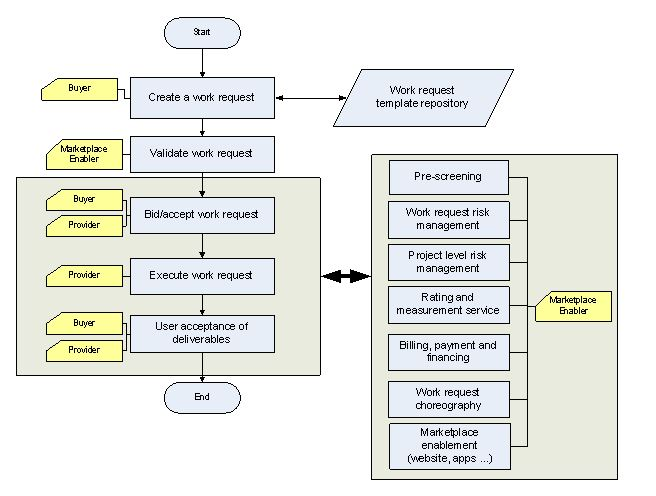
\includegraphics[bb=13 20 530 365, scale=0.53]{figs/glomarketplace.jpg}
\vspace*{-15pt}
\caption{Conceptual illustration of a distributed services marketplace.}
\vspace*{-15pt}
\label{glomarketplace}
\end{figure}

Theoretical analysis can point to optimal regimes and controls for the efficient
use of a services marketplace. For example, Ranade and
Varshney~\cite{glo-ranade} use game-theoretic models to offer insights into some
key questions about crowd-sourcing in general: what type of tasks should be
crowd-sourced and under what circumstances? Their conclusion is that the types
of tasks (specialized or generic) and the distribution of skills in the
available pool of people has a big impact on what can be effectively outsourced.




